\documentclass[tikz,border=5mm]{standalone}
\usetikzlibrary{patterns,backgrounds}

\begin{document}
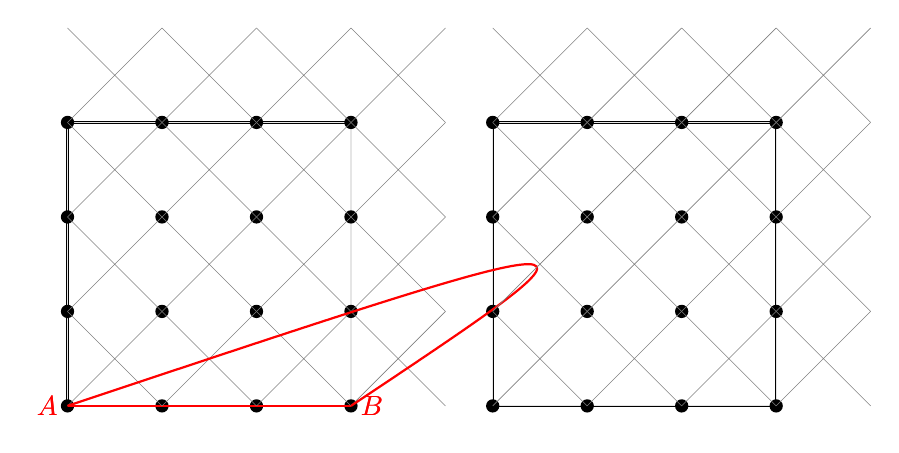
\begin{tikzpicture}[scale=1.2]

% Define grid dimensions
\def\width{3}
\def\height{3}

% Define coordinates for A and B
\coordinate (A) at (0,0);
\coordinate (B) at (\width,0);

% Draw the bounding box
\draw [thick] (0,0) rectangle (\width,\height);

% Fill the background with a light gray pattern
\filldraw[gray!20, even odd rule]
  (0,0) rectangle (\width,\height)
  [pattern=north east lines, pattern color=gray!40] (0,0) rectangle (\width,\height);

% Draw the lattice points
\foreach \x in {0,...,\width} {
    \foreach \y in {0,...,\height} {
        \fill (\x,\y) circle (2pt);
    }
}

% Draw the straight line cut L (AB)
\draw [red, thick] (A) -- (B);

% Label points A and B
\node [left, red] at (A) {$A$};
\node [right, red] at (B) {$B$};

% Connect all lattice points with diagonal lines
\foreach \x in {0,...,\width} {
    \foreach \y in {0,...,\height} {
        \draw [gray, very thin] (\x,\y) -- (\x+1,\y+1) (\x+1,\y) -- (\x,\y+1);
    }
}

% Right figure: Curved cut
\begin{scope}[shift={(4.5,0)}]
    % Draw the bounding box
    \draw [thick] (0,0) rectangle (\width,\height);

    % Fill the background with a light gray pattern
    \filldraw[gray!20, even odd rule]
      (0,0) rectangle (\width,\height)
      [pattern=north east lines, pattern color=gray!40] (0,0) rectangle (\width,\height);

    % Draw the lattice points
    \foreach \x in {0,...,\width} {
        \foreach \y in {0,...,\height} {
            \fill (\x,\y) circle (2pt);
        }
    }

    % Draw the curved line cut L (AB)
    \draw [red, thick] (A) .. controls (\width/2,{\height/2+0.5}) .. (B);

    % Label points A and B
    \node [left, red] at (A) {$A$};
    \node [right, red] at (B) {$B$};

    % Connect all lattice points with diagonal lines
    \foreach \x in {0,...,\width} {
        \foreach \y in {0,...,\height} {
            \draw [gray, very thin] (\x,\y) -- (\x+1,\y+1) (\x+1,\y) -- (\x,\y+1);
        }
    }
\end{scope}

\end{tikzpicture}
\end{document}